\section{协作模式}

\begin{frame}{TBD}{Trunk-Based Development}
    \centering
    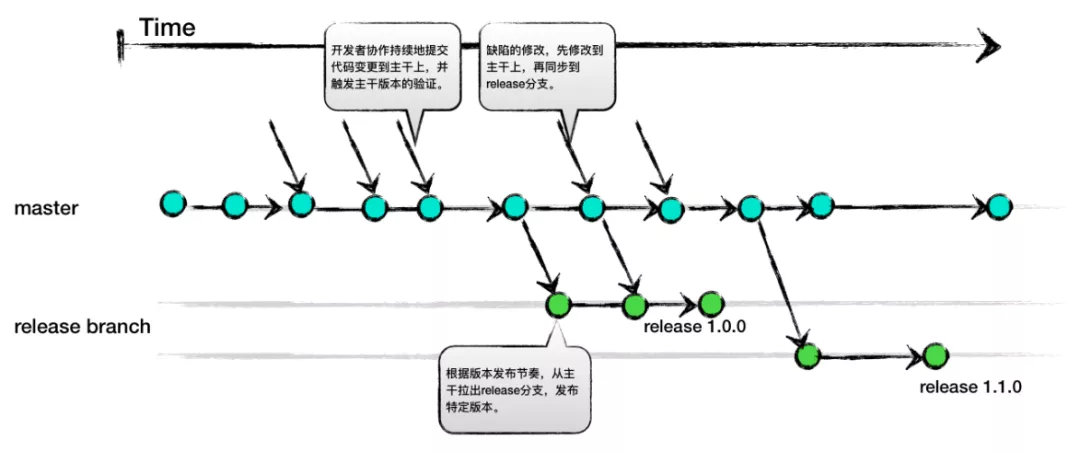
\includegraphics[height=30ex,width=48ex]{figures/tbd.png}
\end{frame}

\begin{frame}[t]{TBD}{优缺点}
    \begin{columns}[onlytextwidth]
        \column{.2\textwidth}
        \column{.6\textwidth}
        \begin{alertblock}{优点}
            \begin{itemize}
                \item 分支少
                \item 操作简单
            \end{itemize}
        \end{alertblock}
        \begin{exampleblock}{缺点}
            \begin{itemize}
                \item 并行开发支持度低
                \item 仅适用于简单版本控制场景
            \end{itemize}
        \end{exampleblock}
        \column{.2\textwidth}
    \end{columns}
\end{frame}

\begin{frame}{Git-Flow}
    \centering
    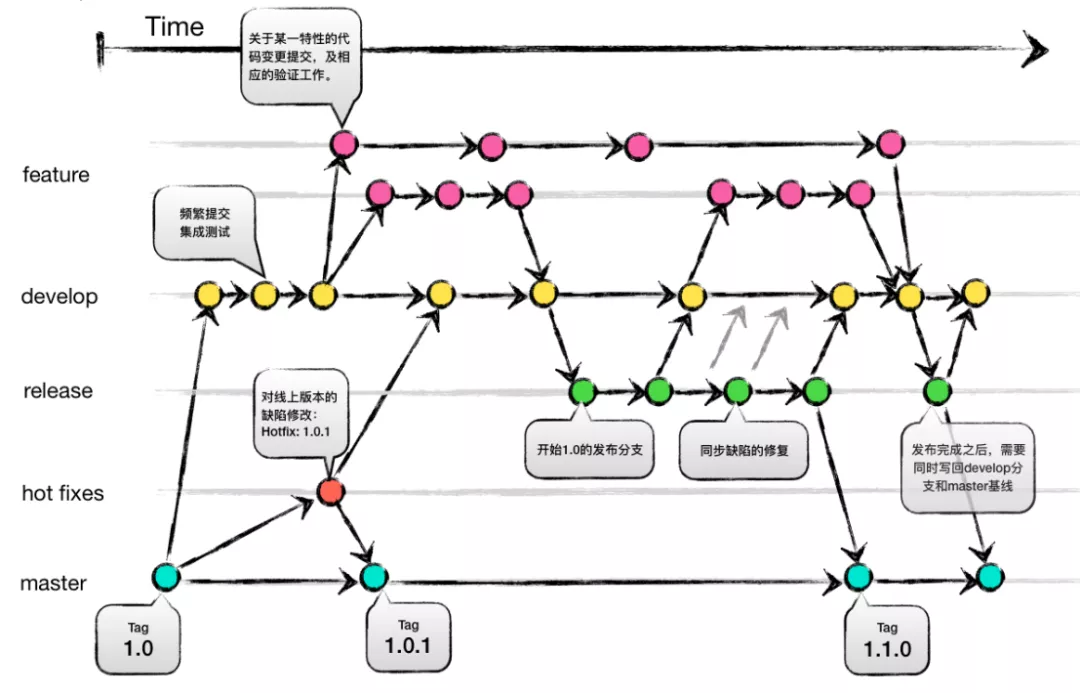
\includegraphics[height=30ex,width=48ex]{figures/git-flow.png}
\end{frame}

\begin{frame}[t]{Git-Flow}{优缺点}
    \begin{columns}[onlytextwidth]
        \column{.2\textwidth}
        \column{.6\textwidth}
        \begin{alertblock}{优点}
            \begin{itemize}
                \item 分支职责清晰
                \item 完善的并行开发支持
                \item 适用于大项目大团队场景
            \end{itemize}
        \end{alertblock}
        \begin{exampleblock}{缺点}
            \begin{itemize}
                \item 分支多
                \item 代码冲突概率大
            \end{itemize}
        \end{exampleblock}
        \column{.2\textwidth}
    \end{columns}
\end{frame}

\begin{frame}{GitHub-Flow}
    \centering
    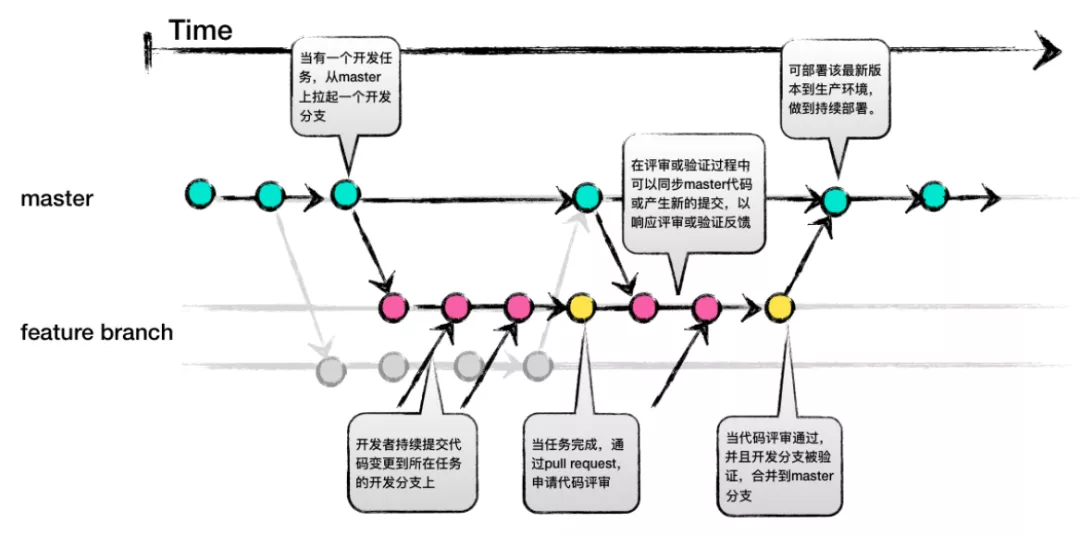
\includegraphics[height=30ex,width=48ex]{figures/github-flow.png}
\end{frame}

\begin{frame}[t]{GitHub-Flow}{优缺点}
    \begin{columns}[onlytextwidth]
        \column{.2\textwidth}
        \column{.6\textwidth}
        \begin{alertblock}{优点}
            \begin{itemize}
                \item 分支逻辑简单
                \item 较高的并行开发支持
                \item 方便与\en{CI/CD}系统集成
            \end{itemize}
        \end{alertblock}
        \begin{exampleblock}{缺点}
            \begin{itemize}
                \item 分支管理不够严谨
            \end{itemize}
        \end{exampleblock}
        \column{.2\textwidth}
    \end{columns}
\end{frame}

\begin{frame}{GitLab-Flow}
    \centering
    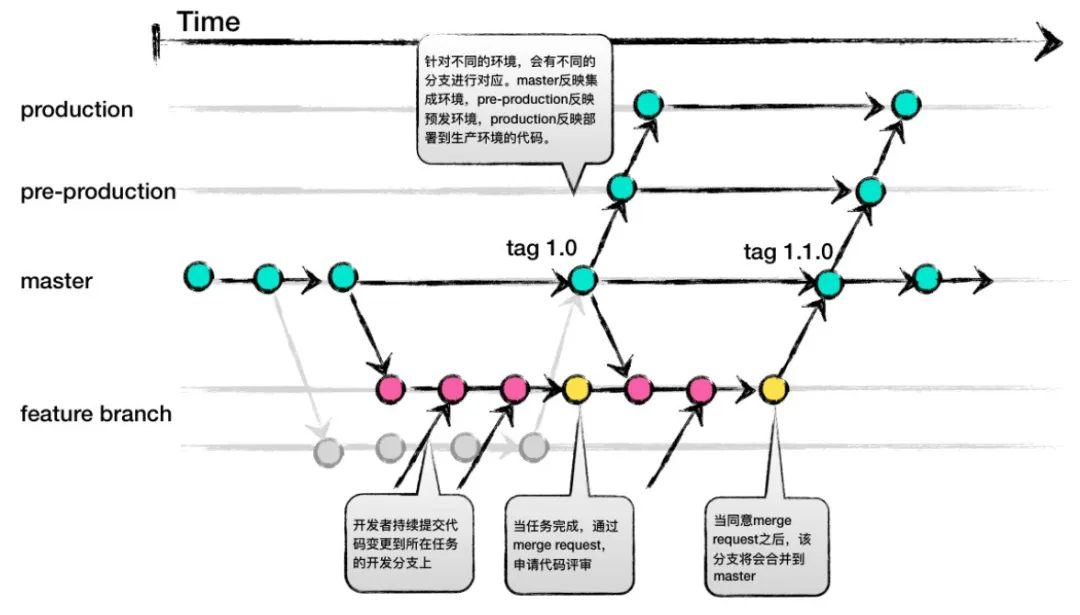
\includegraphics[height=30ex,width=48ex]{figures/gitlab-flow.png}
\end{frame}

\begin{frame}[t]{GitLab-Flow}{优缺点}
    \begin{columns}[onlytextwidth]
        \column{.2\textwidth}
        \column{.6\textwidth}
        \begin{alertblock}{优点}
            \begin{itemize}
                \item 分支管理较严谨
                \item 较高的并行开发支持
                \item 方便与\en{CI/CD}系统集成
            \end{itemize}
        \end{alertblock}
        \begin{exampleblock}{缺点}
            \begin{itemize}
                \item 分支与布署环境过度耦合
                \item 是一种折中方案,复杂度较高
            \end{itemize}
        \end{exampleblock}
        \column{.2\textwidth}
    \end{columns}
\end{frame}